\begin{figure}[h!]
    \centering
    \caption{How stack algorithms work with differing cache sizes}
    \label{fig:my_label}
\begin{tikzpicture}
 \node[rectangle,draw,  minimum width = 2.9cm, 
    minimum height = 1.1cm, label=above:K-1] (r) at (0,0) {
    };
    \node[rectangle,draw,  minimum width = 3.8cm, 
    minimum height = 2.3cm, label=above:K] (t) at (.4,0) {
    };
    \node[rectangle,draw,  minimum width = 4.8cm, 
    minimum height = 3.3cm, label=above:K+1] (u) at (.9,0) {
    };
    \node[rectangle,draw,  minimum width = 6.2cm, 
    minimum height = 4.5cm, label=above:K+2] (p) at (1.6,0) {
    };
\node[rectangle,draw, minimum width = 4cm, 
    minimum height = 1cm,below right = -0.5cm and -1.5cm of r] (q) at (0,0) {
    \begin{tikzpicture}
            \node[rounded corners,draw=black,minimum size=0.8cm]{a};
    \end{tikzpicture}
    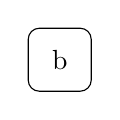
\begin{tikzpicture}
        \node[rounded corners,draw=black,minimum size=0.8cm]{b};
    \end{tikzpicture}
    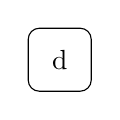
\begin{tikzpicture}
        \node[rounded corners,draw=black,minimum size=0.8cm]{d};
    \end{tikzpicture}
    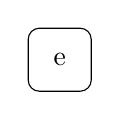
\begin{tikzpicture}
        \node[rounded corners,draw=black, minimum size=0.8cm]{e};
    \end{tikzpicture}
    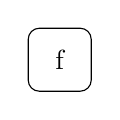
\begin{tikzpicture}
            \node[rounded corners,draw=black,minimum size=0.8cm]{f};
    \end{tikzpicture}
    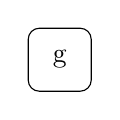
\begin{tikzpicture}
        \node[rounded corners,draw=black,minimum size=0.8cm]{g};
    \end{tikzpicture}
    };
\end{tikzpicture}
\end{figure}